\documentclass{jsarticle}

\usepackage[top=30mm, bottom=36mm, left=28mm, right=28mm]{geometry}
\usepackage[yyyymmdd]{datetime}
\usepackage[dvipdfmx]{graphicx}
\usepackage[subrefformat=parens]{subcaption}
\usepackage{listings}

\usepackage{../common/mytitle}

\title{データ解析特論 第6回}
\author{201720690 小松 弘人}
\date{\today}
\pagestyle{empty}

\makeatletter
\def\mojiparline#1{
    \newcounter{mpl}
    \setcounter{mpl}{#1}
    \@tempdima=\linewidth
    \advance\@tempdima by-\value{mpl}zw
    \addtocounter{mpl}{-1}
    \divide\@tempdima by \value{mpl}
    \advance\kanjiskip by\@tempdima
    \advance\parindent by\@tempdima
}
\makeatother
\def\linesparpage#1{
    \baselineskip=\textheight
    \divide\baselineskip by #1
}

\begin{document}
\maketitle
\thispagestyle{empty}
\subsection*{検討する仮説}
コンクリート構造物をハンマーで叩き、その反響音から内部の欠陥を
検出する打音法と呼ばれる検査手法の研究が盛んに行われている。
現在は、欠陥部を叩いた反響音と健全部を叩いた反響音を機械学習により学習させることで
内部の欠陥が検出できるかどうかを検証している。
しかし、様々な深さ・大きさの欠陥を分類して学習を行うと非常に多くの時間がかかることが分かっている。
そこで、学習の過程をFPGAにより高速化することで、学習時間を短縮したい。

FPGAで実装するにあたり、入力データの次元数はできるだけ削減したい。
そこで、入力データに対し主成分分析をすることを考えた。
今回は、主成分分析したデータを入力として用いることによりクラス分類のエラー率が変化しないことを検証する。
そのために、線形回帰によるクラス分類を行い、その正確度の平均に有意な差がないことを\emph{t}検定を用いて確認する。

\subsection*{対象とするデータ}

今回は、供試体上の様々な欠陥モデルから収集したデータのうち、
直径が$100\mathrm{[mm]}$、表層からの深さが$40\mathrm{[mm]}$の
欠陥モデルから得られたデータを用いる。
このデータには、欠陥モデル上を叩いて得られた反響音 (欠陥部) と
その周囲を叩いて得られた反響音 (健全部) が含まれる。
それぞれのクラスのデータ数は、欠陥部が509個、健全部が526個である。

従来手法では、反響音に対し、サンプル数512でFFTを行ったものを入力データとして用いている。
今回は、このFFTを行ったデータに対して主成分分析を行い、
寄与率が高い主成分から順に取り出したものを新たな入力データとして用いることを考える。
新たな入力データは、主成分の寄与率の合計が$99.9\%$を超える第54主成分までを用いる。

\subsection*{前処理}

今回使用するデータは、欠損がないことが分かっているため、欠損値に対する処理は不必要である。
ただし、スクリプトでは念のため欠損がないことを確認する。

それぞれのデータに対し、箱ひげ図をプロットした (図\ref{img:box})。
次元数が多いため細部は見えにくいが、欠陥部、健全部ともに
外れ値と思われる値が存在することが確認できる。
そこで、1クラスSVMを使った外れ値検出を行う。
カーネルは線形カーネルを用いる。
箱ひげ図より、欠陥部は外れ値が20個程度であると考えられるため$\nu=0.04$とし、
健全部はそれより少し多いと考え$\nu=0.05$とした。

\begin{figure}[htbp]
	\centering
	\begin{minipage}{.8\hsize}
		\centering
		\begin{tabular}{c}
			\begin{minipage}{0.5\hsize}
				\centering
                \includegraphics[width=\linewidth]{img/fftD.pdf}
                \subcaption{FFT(欠陥部)}
			\end{minipage}
			\begin{minipage}{0.5\hsize}
				\centering
				\includegraphics[width=\linewidth]{img/fftH.pdf}
				\subcaption{FFT(健全部)}
			\end{minipage}
		\end{tabular}
	\end{minipage}
	\begin{minipage}{.8\hsize}
		\centering
		\begin{tabular}{c}
			\begin{minipage}{0.5\hsize}
				\centering
				\includegraphics[width=\linewidth]{img/pcaD.pdf}
				\subcaption{PCA(欠陥部)}
			\end{minipage}
			\begin{minipage}{0.5\hsize}
				\centering
				\includegraphics[width=\linewidth]{img/pcaH.pdf}
				\subcaption{PCA(健全部)}
			\end{minipage}
		\end{tabular}
	\end{minipage}
    \caption{箱ひげ図}
    \label{img:box}
\end{figure}

\begin{figure}[htbp]
    \centering
    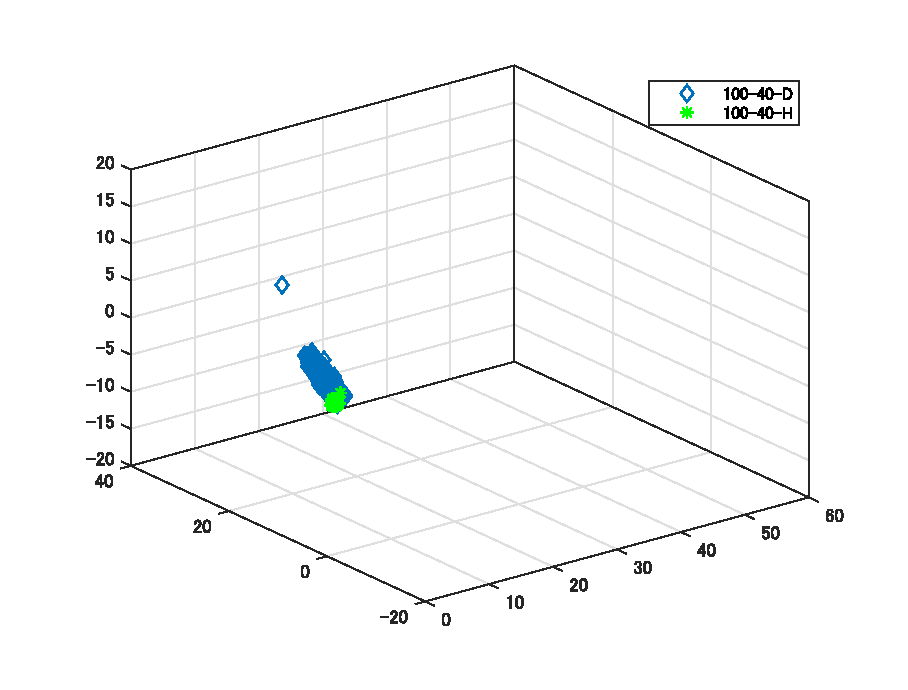
\includegraphics[width=.5\linewidth]{img/100-40.eps}
    \caption{$\phi$100-40のデータの3次元空間への射影}
    \label{img:100-40}
\end{figure}

\subsection*{知識発見の処理}
直径100[mm]、深さ40[mm]の欠陥モデルから得られるデータを
第1、第2、第3主成分から張られる空間に射影すると、図\ref{img:100-40}のようになることが分かっている。
そこで、従来の入力データおよび新しい入力データのそれぞれに対し
線形回帰を行い、所属するクラスを推測させ、その正確度を求めた。

このとき、欠陥部のデータのクラスを1、健全部のデータのクラスを2とする。
今回は、クラス分類であることから、線形回帰の推測値を四捨五入した。
また、クロスバリデーションの分割数を$k=10$とした。

\subsection*{結果の正当性の検証}
主成分分析をする前とした後で、10回の試行における正確度の平均が変わらないことを確認するため
\emph{t}検定を行う。
また、外れ値の処理をする前とした後の正確度についても、同様に検定を行う。
\emph{t}検定は両側検定で行い、信頼区間は$95\%$とする。

まず、外れ値の処理をするか否かによる正確度への影響を確認するためのスクリプトの実行結果を示す。
上が従来の入力データについてであり、下が新しい入力データについての検定の結果である。
検定の結果を表\ref{tbl:outlier}にまとめる。

\begin{lstlisting}[basicstyle=\ttfamily\footnotesize, frame=single]
        Welch Two Sample t-test

data:  errFFTAll and errFFTOR
t = 0, df = 18, p-value = 1
alternative hypothesis: true difference in means is not equal to 0
95 percent confidence interval:
 -0.01143062  0.01143062
sample estimates:
mean of x mean of y
0.9942214 0.9942214


        Welch Two Sample t-test

data:  errPCAAll and errPCAOR
t = 0, df = 18, p-value = 1
alternative hypothesis: true difference in means is not equal to 0
95 percent confidence interval:
 -0.008936802  0.008936802
sample estimates:
mean of x mean of y
0.9951264 0.9951264
\end{lstlisting}

\begin{table}
	\centering
	\caption{\emph{t}検定の結果 (外れ値の処理の有無)}
	\label{tbl:outlier}
	\begin{tabular}{c||c|c|c|c}
		\hline
		Input & mean of x & mean of y & t値 & p-value \\ \hline \hline
		FFT & 0.9942214 & 0.9942214 & 0 & 1 \\ \hline
		PCA & 0.9951264 & 0.9951264 & 0 & 1 \\ \hline
	\end{tabular}
\end{table}

次に、外れ値の処理をしたデータについて、主成分分析をする前とした後の正確度が変化するかを
検定した結果を以下に示す。
また、検定の結果を表\ref{tbl:cmp}にまとめる。
\begin{lstlisting}[basicstyle=\ttfamily\footnotesize, frame=single]
        Welch Two Sample t-test

data:  errFFTOR and errPCAOR
t = -0.18531, df = 17.01, p-value = 0.8552
alternative hypothesis: true difference in means is not equal to 0
95 percent confidence interval:
 -0.011207720  0.009397765
sample estimates:
mean of x mean of y
0.9942214 0.9951264
\end{lstlisting}

\begin{table}
	\centering
	\caption{\emph{t}検定の結果 (主成分分析の有無)}
	\label{tbl:cmp}
	\begin{tabular}{c|c|c|c}
		\hline
		mean of FFT & mean of PCA & t値 & p-value \\ \hline \hline
		0.9942214 & 0.9951264 & -0.18531 & 0.8552 \\ \hline
	\end{tabular}
\end{table}

\subsection*{考察}
帰無仮説は「2つの正確度の平均の差は0である」である。
表\ref{tbl:outlier}より、p値が1であるため、帰無仮説は棄却できない。
むしろ、今回のデータにおいては平均の差は0であるといえる。
これは、線形回帰によって推測されたクラスの値を四捨五入したためであると考えられる。
したがって、今回のデータについては外れ値を排除しても
正確度に有意な差は得られないことが確認できる。

また、表\ref{tbl:cmp}より、p値が0.8552であるため、帰無仮説は棄却できない。
したがって、主成分分析を行う前と後の正確度の平均は有意な差があるとはいえない。
よって、主成分分析を行ったデータを入力とすることによる正確度への影響は決して大きくはないといえる。

\subsection*{結論}
直径100[mm]、深さ40[mm]の欠陥については、主成分分析によって入力データの次元を削減しても
正確度への影響は小さいことが確認できた。
したがって、主成分分析による入力データの次元の削減は有効であると考えられる。

\end{document}
